% ---------------------------------------------------------------------------
% Figure 3. The seven-role elite decision chain under a civilian and a
% military constitution.
%
% RE-BASED, 2026-11-25. The submitted version of this figure showed the chain
% "under Scenario A (civilian)". Scenario A is the self-designed constitution
% and has been dropped from the reported roster, so a figure resting on it can
% no longer appear. This version shows the two REAL, historically enacted
% constitutions that now carry the differential-constraint claim: South Korea's
% 1987 constitution (civilian chain) and Pakistan's 1973 constitution as
% amended by Zia's 8th Amendment of 1985 (military chain).
%
% VERIFIED AGAINST LIVE SOURCE, 2026-11-25:
%   * chain structure .... engine/elite_agents_v3.py, CHAIN_ORDER_CIVILIAN and
%                          CHAIN_ORDER_MILITARY (lines 90-108). The seven
%                          role-function slots and their order are properties
%                          of chain_type, not of the country.
%   * country titles ..... AGENT_DISPLAY_NAMES_BY_SCENARIO, read back through
%                          the module rather than transcribed by hand.
%   * chain_type ......... config/scenario_registry.py: SK civilian, PK military.
%
% NO COUNTS APPEAR IN THIS FIGURE, DELIBERATELY. The interception and emission
% totals currently available are smoke-test lower bounds on superseded code.
% The figure asserts the mechanism, which is structural; magnitudes belong in a
% table that the campaign will populate.
% ---------------------------------------------------------------------------
\documentclass[border=10pt]{standalone}
% ---------------------------------------------------------------------------
% kanova-figstyle.tex
% Single source of truth for the visual style of every Ka-Nova figure.
%
% Reviewer 1, concern 6 asked that "fonts, labels, symbols, line weights, and
% overall graphical style" be made consistent across figures. Every schematic
% inputs this file and defines no local colours, line widths or fonts, so the
% consistency is structural rather than something maintained by eye.
%
% Design constraints, all deliberate:
%   * Vector output only. No raster element appears in any figure.
%   * Greyscale safe. IEEE Access prints in colour but is read in greyscale.
%     Civilian and military elements are separated by fill LIGHTNESS and by
%     border dash pattern, never by hue alone, so the distinction survives a
%     monochrome printer.
%   * Sans-serif labels at 8 pt, per the IEEE Author Center guidance for
%     figure text, applied identically in all four figures.
%   * Three line weights only, listed below. No figure introduces a fourth.
% ---------------------------------------------------------------------------

\usepackage{tikz}
\usetikzlibrary{arrows.meta,positioning,calc,fit,backgrounds,shapes.geometric,%
                decorations.pathreplacing,shapes.symbols,shapes.multipart}
\usepackage[scaled=0.92]{helvet}
\renewcommand{\familydefault}{\sfdefault}

% --- Palette. Lightness values chosen to stay distinguishable in greyscale. --
\definecolor{knink}{RGB}{26,26,26}        % all text and borders
\definecolor{knrule}{RGB}{120,120,120}    % secondary rules, annotations
\definecolor{knfillA}{RGB}{244,244,244}   % lightest  structural / container
\definecolor{knfillB}{RGB}{232,236,241}   % light     engine / mechanism
\definecolor{knfillC}{RGB}{214,222,232}   % mid       constitutional layer
\definecolor{knciv}{RGB}{226,235,228}     % civilian  chain  (lighter)
\definecolor{knmil}{RGB}{206,206,206}     % military  chain  (darker)
\definecolor{knaccent}{RGB}{140,30,30}    % CVES interception, used sparingly
\definecolor{knstore}{RGB}{250,246,235}   % persisted artefact

% --- The only three line weights used anywhere. ----------------------------
\newcommand{\knthin}{0.4pt}
\newcommand{\knnorm}{0.7pt}
\newcommand{\knbold}{1.1pt}

% --- Typography inside figures. -------------------------------------------
\newcommand{\knlabel}[1]{{\fontsize{8}{9.6}\selectfont #1}}
\newcommand{\knsmall}[1]{{\fontsize{7}{8.4}\selectfont #1}}
\newcommand{\kntiny}[1]{{\fontsize{6}{7.2}\selectfont #1}}
\newcommand{\knhead}[1]{{\fontsize{8}{9.6}\selectfont\bfseries #1}}
\newcommand{\kncode}[1]{{\fontsize{7}{8.4}\selectfont\ttfamily #1}}

\tikzset{
  every node/.style     = {font=\fontsize{8}{9.6}\selectfont, text=knink,
                           align=center, inner sep=3pt},
  % process / component box
  knbox/.style          = {draw=knink, line width=\knnorm, fill=knfillB,
                           rounded corners=1.5pt, minimum height=7mm,
                           inner xsep=4pt, inner ysep=3pt},
  % constitutional layer box
  knconst/.style        = {knbox, fill=knfillC},
  % passive container / grouping
  kngroup/.style        = {draw=knrule, line width=\knthin, fill=knfillA,
                           rounded corners=2.5pt, dash pattern=on 2pt off 1.5pt,
                           inner sep=6pt},
  % persisted artefact on disk
  knfile/.style         = {draw=knink, line width=\knnorm, fill=knstore,
                           rounded corners=0pt, minimum height=6.5mm,
                           inner xsep=4pt},
  % civilian elite role: lighter fill, solid border
  knrolec/.style        = {draw=knink, line width=\knnorm, fill=knciv,
                           rounded corners=1.5pt, minimum height=6mm,
                           minimum width=42mm, inner xsep=3pt, inner ysep=2pt},
  % military elite role: darker fill, dashed border. Two cues, not one.
  knrolem/.style        = {draw=knink, line width=\knnorm, fill=knmil,
                           rounded corners=1.5pt, dash pattern=on 3pt off 1.5pt,
                           minimum height=6mm, minimum width=42mm,
                           inner xsep=3pt, inner ysep=2pt},
  % CVES validation layer
  knlayer/.style        = {draw=knink, line width=\knnorm, fill=knfillB,
                           rounded corners=1.5pt, minimum height=8mm,
                           minimum width=30mm},
  % decision point
  kndec/.style          = {draw=knink, line width=\knnorm, fill=knfillA,
                           diamond, aspect=2.4, inner sep=1.5pt},
  % numbered step marker
  knstep/.style         = {draw=knink, line width=\knnorm, fill=white,
                           circle, inner sep=0pt, minimum size=4.6mm,
                           font=\fontsize{7}{7}\selectfont\bfseries},
  % --- edges. One arrow tip shape in the whole figure set. ----------------
  knflow/.style         = {draw=knink, line width=\knnorm,
                           -{Stealth[length=1.9mm, width=1.4mm]}},
  knflowbold/.style     = {knflow, line width=\knbold},
  knread/.style         = {draw=knrule, line width=\knthin,
                           dash pattern=on 1.5pt off 1.5pt,
                           -{Stealth[length=1.6mm, width=1.2mm]}},
  knblock/.style        = {draw=knaccent, line width=\knbold,
                           -{Bar[width=2.2mm]}},
  knnote/.style         = {font=\fontsize{6}{7.2}\selectfont, text=knrule,
                           align=left, inner sep=1.5pt},
  % panel / section heading, bold at body size
  knpanelhead/.style    = {font=\fontsize{8}{9.6}\selectfont\bfseries,
                           text=knink, align=center, inner sep=2pt},
}

\begin{document}
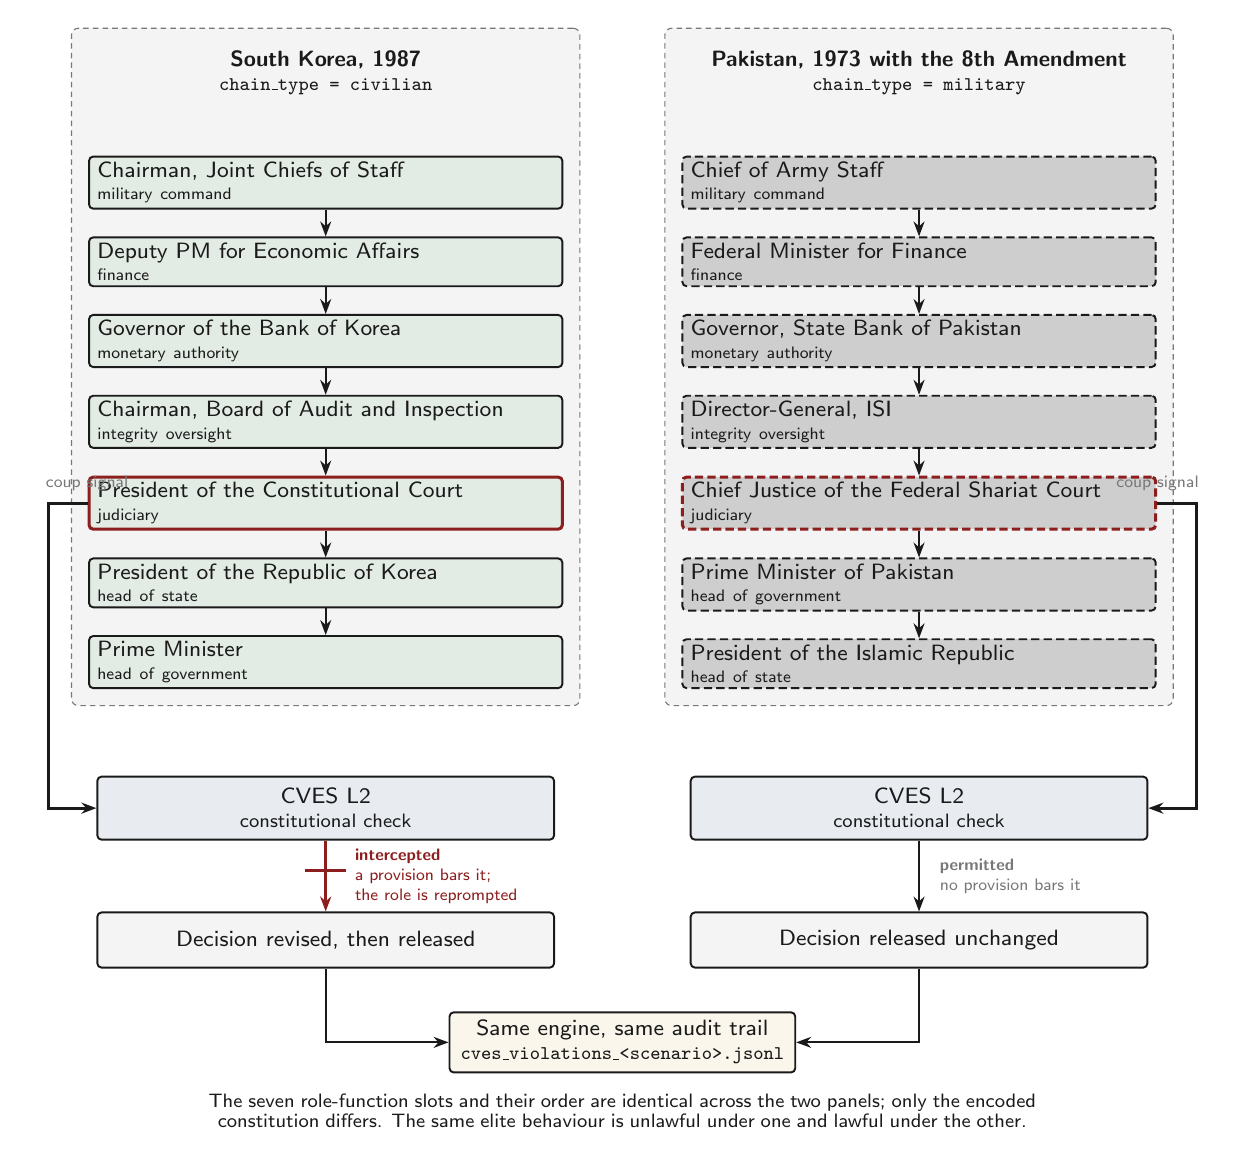
\begin{tikzpicture}

\def\rw{58mm}      % role box width
\def\gap{15mm}     % gap between the two panels
\tikzset{
  rc/.style={knrolec, text width=\rw, align=left, minimum width=0pt},
  rm/.style={knrolem, text width=\rw, align=left, minimum width=0pt},
}
\newcommand{\role}[2]{\knlabel{#1}\\[-1.5pt]\kntiny{#2}}

% ===== LEFT PANEL, South Korea 1987, civilian chain ========================
\node[rc] (a1) {\role{Chairman, Joint Chiefs of Staff}{military command}};
\node[rc, below=3.4mm of a1] (a2) {\role{Deputy PM for Economic Affairs}{finance}};
\node[rc, below=3.4mm of a2] (a3) {\role{Governor of the Bank of Korea}{monetary authority}};
\node[rc, below=3.4mm of a3] (a4) {\role{Chairman, Board of Audit and Inspection}{integrity oversight}};
\node[rc, below=3.4mm of a4, draw=knaccent, line width=\knbold] (a5) {\role{President of the Constitutional Court}{judiciary}};
\node[rc, below=3.4mm of a5] (a6) {\role{President of the Republic of Korea}{head of state}};
\node[rc, below=3.4mm of a6] (a7) {\role{Prime Minister}{head of government}};

% ===== RIGHT PANEL, Pakistan 1973 + 8th Amendment, military chain ==========
\node[rm, right=\gap of a1] (b1) {\role{Chief of Army Staff}{military command}};
\node[rm, below=3.4mm of b1] (b2) {\role{Federal Minister for Finance}{finance}};
\node[rm, below=3.4mm of b2] (b3) {\role{Governor, State Bank of Pakistan}{monetary authority}};
\node[rm, below=3.4mm of b3] (b4) {\role{Director-General, ISI}{integrity oversight}};
\node[rm, below=3.4mm of b4, draw=knaccent, line width=\knbold] (b5) {\role{Chief Justice of the Federal Shariat Court}{judiciary}};
\node[rm, below=3.4mm of b5] (b6) {\role{Prime Minister of Pakistan}{head of government}};
\node[rm, below=3.4mm of b6] (b7) {\role{President of the Islamic Republic}{head of state}};

% ===== sequential chain edges =============================================
\foreach \a/\b in {a1/a2,a2/a3,a3/a4,a4/a5,a5/a6,a6/a7} {\draw[knflow] (\a) -- (\b);}
\foreach \a/\b in {b1/b2,b2/b3,b3/b4,b4/b5,b5/b6,b6/b7} {\draw[knflow] (\a) -- (\b);}

% ===== panel headings ======================================================
\node[knpanelhead, above=7mm of a1.north, anchor=south] (ha)
  {South Korea, 1987\\[-1pt]\knsmall{\texttt{chain\_type = civilian}}};
\node[knpanelhead, above=7mm of b1.north, anchor=south] (hb)
  {Pakistan, 1973 with the 8th Amendment\\[-1pt]\knsmall{\texttt{chain\_type = military}}};

\begin{scope}[on background layer]
  \node[kngroup, fit=(ha)(a1)(a7)] (panA) {};
  \node[kngroup, fit=(hb)(b1)(b7)] (panB) {};
\end{scope}

% ===== the mechanism: identical signal, opposite constitutional treatment ==
\node[knlayer, below=11mm of a7, minimum width=\rw, fill=knfillB] (cvA)
  {\knlabel{CVES L2}\\[-1pt]\knsmall{constitutional check}};
\node[knlayer, below=11mm of b7, minimum width=\rw, fill=knfillB] (cvB)
  {\knlabel{CVES L2}\\[-1pt]\knsmall{constitutional check}};

\draw[knflowbold] (a5.west) -- ++(-5mm,0)
   node[knnote, anchor=south west, yshift=0.8mm, xshift=-1mm] {coup signal}
   |- ($(cvA.west)+(-5mm,0)$) -- (cvA.west);
\draw[knflowbold] (b5.east) -- ++(5mm,0)
   node[knnote, anchor=south east, yshift=0.8mm, xshift=1mm] {coup signal}
   |- ($(cvB.east)+(5mm,0)$) -- (cvB.east);

\node[knbox, below=9mm of cvA, minimum width=\rw, fill=knfillA] (outA)
  {\knlabel{Decision revised, then released}};
\node[knbox, below=9mm of cvB, minimum width=\rw, fill=knfillA] (outB)
  {\knlabel{Decision released unchanged}};

\draw[knflow, draw=knaccent, line width=\knbold] (cvA) --
  node[knnote, anchor=west, xshift=3mm, text=knaccent]
  {\textbf{intercepted}\\a provision bars it;\\the role is reprompted} (outA);
\draw[draw=knaccent, line width=\knbold]
  ($(cvA.south)!0.42!(outA.north)+(-2.6mm,0)$) --
  ($(cvA.south)!0.42!(outA.north)+(2.6mm,0)$);
\draw[knflow] (cvB) -- node[knnote, anchor=west, xshift=2mm]
  {\textbf{permitted}\\no provision bars it} (outB);

\node[knbox, fill=knstore, minimum width=40mm] (trail) at
  ($(outA)!0.5!(outB) + (0,-13mm)$)
  {\knlabel{Same engine, same audit trail}\\[-1pt]\kncode{cves\_violations\_<scenario>.jsonl}};
\draw[knflow] (outA.south) |- (trail.west);
\draw[knflow] (outB.south) |- (trail.east);

\node[knnote, anchor=north, text width=150mm, align=center, text=knink]
  at ($(trail.south)+(0,-2mm)$)
  {\knsmall{The seven role-function slots and their order are identical across the two
   panels; only the encoded constitution differs. The same elite behaviour is
   unlawful under one and lawful under the other.}};

\end{tikzpicture}
\end{document}
